\section{Literature Review}

\subsection{Factors Affecting Bus Arrival Times}
\label{factors-affecting-arrival-times}

There are a variety of different factors that can affect the arrival time of a bus. be that through affecting the travel time of the bus or the dwell time of the bus. For example, the bus' travel time could be affected by traffic conditions. Similarly, the bus' dwell time (the time that it spends at a bus stop before it can continue on its route) could be affected if there are a large number of people that get on at the previous stop. Due to the sheer number of factors that could be investigated, this section will take a brief look at a selection of the factors that have been considered in other papers as well as some other factors that have the potential to be important. This section will also attempt to argue why some of the factors listed below do not warrant further investigation and do not need to be included in the models that will be developed. \\

It should be noted that most of the factors mentioned below are largely dependent upon one another. For example, the time of day could affect the traffic conditions (say rush hour leading to more vehicles on the road) or the weather could affect the traffic conditions (if it is particularly cold and icy, there may be fewer people willing to drive to work, so there are fewer cars on the road). Therefore, care will have to be taken when implementing the models, to ensure that not too much weighting is placed on any singular factor.

\subsubsection{Weather}
\label{weather}
Koetse and Reitveld found that there is a substantial reduction in traffic speed when weather conditions are extreme \cite{weather-transport-effect}. In the presence of rain there was a decrease of up to 6\% in traffic speed, up to 13\% for snow and up to 12\% for reduced visibility. Slower traffic speeds means that vehicles will take longer to arrive at their destinations than usual and therefore, it can be argued that weather should be taken into account when creating models that predict bus arrival times. Furthermore, when temperatures are at the extremes, there is a case for people being more likely to take a bus than walking or cycling. Not only would this increase the load on the bus, leading to a slower bus speed, but the dwell time at the bus stops would also increase as more time would have to be taken for people to get on and off the buses. \\

As mentioned in Section \ref{section:regression-models-research}, it was found by Patnaik et al. that there was little to no effect between weather and bus delay time \cite{apc-estimation}. This finding was attributed to the fact that the weather data used in this investigation was not sufficiently detailed or that during the study period, the weather variations were not significant enough to have an impact on arrival times. Therefore, it is likely that I will not be exploring any further the effect of weather on bus arrival times. All the data that will be used in this project has to be collected manually since TfL does not provide any historical data on bus arrival times, and so most of the collected data would be from the periods spanning mid January to May time. This would not be a large enough sample of different and extreme weather conditions and so, based off of Patnaik et al's findings, this supports the idea that weather would not be very suitable to be studied as a factor affecting bus arrival times in this particular project.

\subsubsection{Time of Day and Time of Week}
\label{time-of-day-week}
At different times of day and different days of the week, there are different travel patterns. For example, at weekday rush hour times, there are more likely to be more vehicles on the road and thus more congestion. On the other hand, on weekends, there is less likely to be a strong correlation between time of day and late buses as there is not a particular time when a large proportion of the population has to travel somewhere. \\

W Fan and Z Gurmu clustered their travel time data by time period and explored the effects of this. The results can be seen in Figure \ref{fig:time-of-day-week}, which plots the travel time index against the time of day for the LT11 line in the Northbound direction in Maca\'e, Rio de Janeiro, Brazil \cite{dynamic-gps}. Here, the travel time index is the ratio of the average travel time per weekday and the average travel time across all days. An observation that was made was that in the evening rush hour (5 - 6 pm), the travel times were 30\% higher than the average across all time periods and days. This supports the idea of further exploring time of day as a parameter in the predicting of bus arrival times. Another observation that was made was that the travel time distributions over the different days of the week seemed to be nearly the same. Therefore, since Figure \ref{fig:time-of-day-week} only shows data for weekdays, it could be argued that for weekdays, it will suffice to look at the effect of the time of day, without taking into account which day of the week it is. A similar concession can be made for weekends, i.e. the prediction model for Saturday 3pm should be no different to the prediction model for Sunday 3pm. However, these assumptions are based on a model for a city in Brazil. It is unclear how strongly these findings would generalise to London. For example, the daily travel landscape, in terms of when people leave work etc. are unlikely to be the same.

\begin{figure}[H]
\begin{center}
    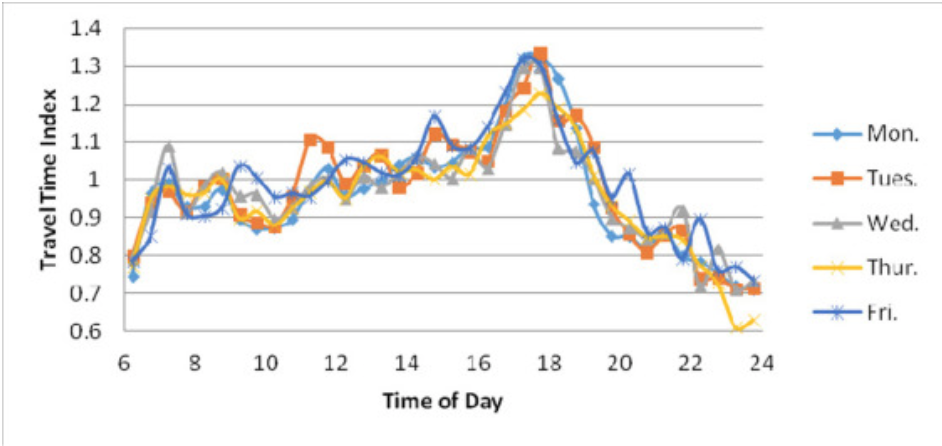
\includegraphics[scale=0.8]{Images/day-time-of-week-effect.png}
    \caption{Effect of time of day and day of week on travel time, original image from \cite{dynamic-gps}}
    \label{fig:time-of-day-week}
\end{center}
\end{figure}

Google studied the delay patterns of buses for a new feature introduced into Google Maps and some of the results can be seen in Figure \ref{fig:week-vs-weekend}, which shows the predicted travel time for a bus ride with traffic held constant \cite{google-machine-learning}. This suggests that travel patterns during the week versus the weekend are different and further supports the idea that the same models can be used for all weekdays whilst a different model should be used for weekends.

\begin{figure}[H]
\begin{center}
    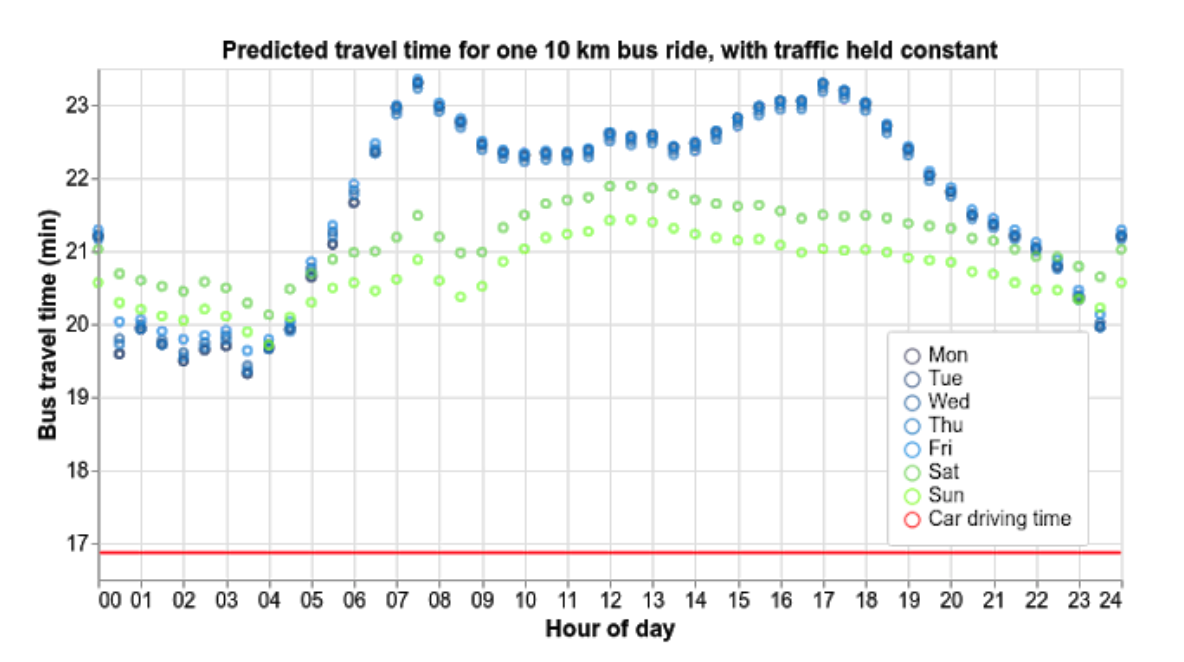
\includegraphics[scale=0.7]{Images/week-weekend.png}
    \caption{How time and day of week affects travel time, original image from \cite{google-machine-learning}}
    \label{fig:week-vs-weekend}
\end{center}
\end{figure}

Based on the above, the effect of time of day and time of week on bus arrival times will be investigated further in my models.

\subsubsection{Time of Year}
Similarly to the previous parameter, at different times of year, there are different travel patterns for buses. This could be due to factors such as special occasion (e.g. New Year's Day or bank holidays) or school holidays. For example, during term time, buses are not likely to have have the same travel time as during school holidays. According to National Travel Survey statistics, 19\% of children aged 5 to 16 travelled to school by bus and 21\% travelled by bus or van in the year 2017/18 \cite{children-school-travel-mode}. Therefore, during term time, there are not only more vehicles on the road, thus increasing the likelihood of congestion, but buses will also have longer dwell times because they will have to wait for children to board and deboard. Therefore, during school holidays when a large number of these children will no longer be making daily regular trips on the bus and there are fewer vehicles on the road, the travel time of a bus may be faster and thus it may be less likely to be delayed. However, in this particular example of school holidays playing a part in predicting bus arrival times, it could be argued that because children travel to school around the same time as rush hour, the effect of this could be explored in the previous parameter: time of day and time of week. \\

Time of year is unlikely to be explored any further as a factor affecting bus arrival times. As mentioned previously, the data used in this project will have to be collected manually and due to time constraints and lack of historical data, it is impossible to get a whole year's worth of data to use for modelling. 

\subsubsection{Dwell Time at Bus Stops}
The amount of time a bus spends at a bus stop before continuing on its journey, also known as its dwell time, is one of the factors that have been considered to affect the arrival time of a bus. The dwell time of a bus can be affected by varying numbers of passengers at bus stops. For example, if a bus stop is outside a particularly popular destination, then the number of passengers getting off the bus would be higher than normal and thus the bus would have to wait at that particular stop for a longer amount of time. \\

In a study that used regression models to look at parameters affecting bus arrival times, it was found that bus stop dwell times were less important and statistically not as significant \cite{dynamic-gps}. Furthermore, with the tools currently available, there is no real way to calculate how long a bus waits a single stop for. TfL does not currently provide any APIs that would directly give a bus' dwell time nor does it provide APIs that could aid in the calculation of dwell time, e.g. the number of passengers boarding or deboarding a bus. Therefore, dwell times of buses will not be taken into account in the models that I will develop. 

\subsubsection{Traffic Conditions}
Jeong and Rilett argued that in order to accurately predict bus travel time, it it essential to consider traffic conditions \cite{ann-prediction}. In June 2019 Google Maps introduced a new feature for forecasting bus delays by taking into account real time car traffic data and combining this with data on bus routes and stops \cite{google-machine-learning}. Both of these support the idea that traffic conditions should be considered as one of the parameters that affect bus arrival times. \\

However, Williams and Hoel found that daily traffic condition patterns were consistent across the weeks \cite{consistent-traffic}. This implies that if bus delays are affected by traffic, then historical bus travel times should not vary across the same time periods for different weeks and therefore, traffic conditions do not need to be taken into account as a factor, especially for historical average models. This is supported by Fan and Gurmu, who argue that if traffic patterns are relatively stable over time, then historical average models will perform well \cite{dynamic-gps}. \\

It can also be argued that the presence of bus only lanes means that there is little point in taking general traffic into account because traffic conditions will have less of an effect on the travel time of buses. Therefore, taking all of the above into account, traffic conditions will only be considered further as a factor affecting bus arrival times if I have time.

\subsubsection{COVID-19 Lockdown in London}

TODO Pre and post lockdown travel conditions -> I have some data from February maybe?

\subsection{Chapter Conclusion}

A chapter conclusion is important. You could reiterate which measures you have chosen to track out of the many possible options you've considered

\subsection{Clustering Analysis}

Clustering methods have been used to investigate typical bus delay information. F Sun, Y Pan, J White and A Dube clustered the travel times of buses by different times of day and discovered that there were different travel patterns over different time periods \cite{smart-public-transport}.

Sun et al. applied the K-means algorithm for each of day of the week to cluster the bus delay data according to delay and time in the day, varying k from 2 to 5. The silhouette score was then calculated on each of the different clusters obtained and the k value that had the best silhouette score was chosen to be the optimal number of clusters. Figure \ref{fig:clustered-historical-data} shows the results of the clustering for the historical delay data of a bus at a particular bus stop on an outbound journey over a 24 hour period on every Tuesday between 01/08/2015 and 31/08/2015. It can be seen that most of the points are roughly clustered into the green and blue groups, suggesting two different delay patterns: one before 1230 and one after. 

\begin{figure}[H]
\begin{center}
    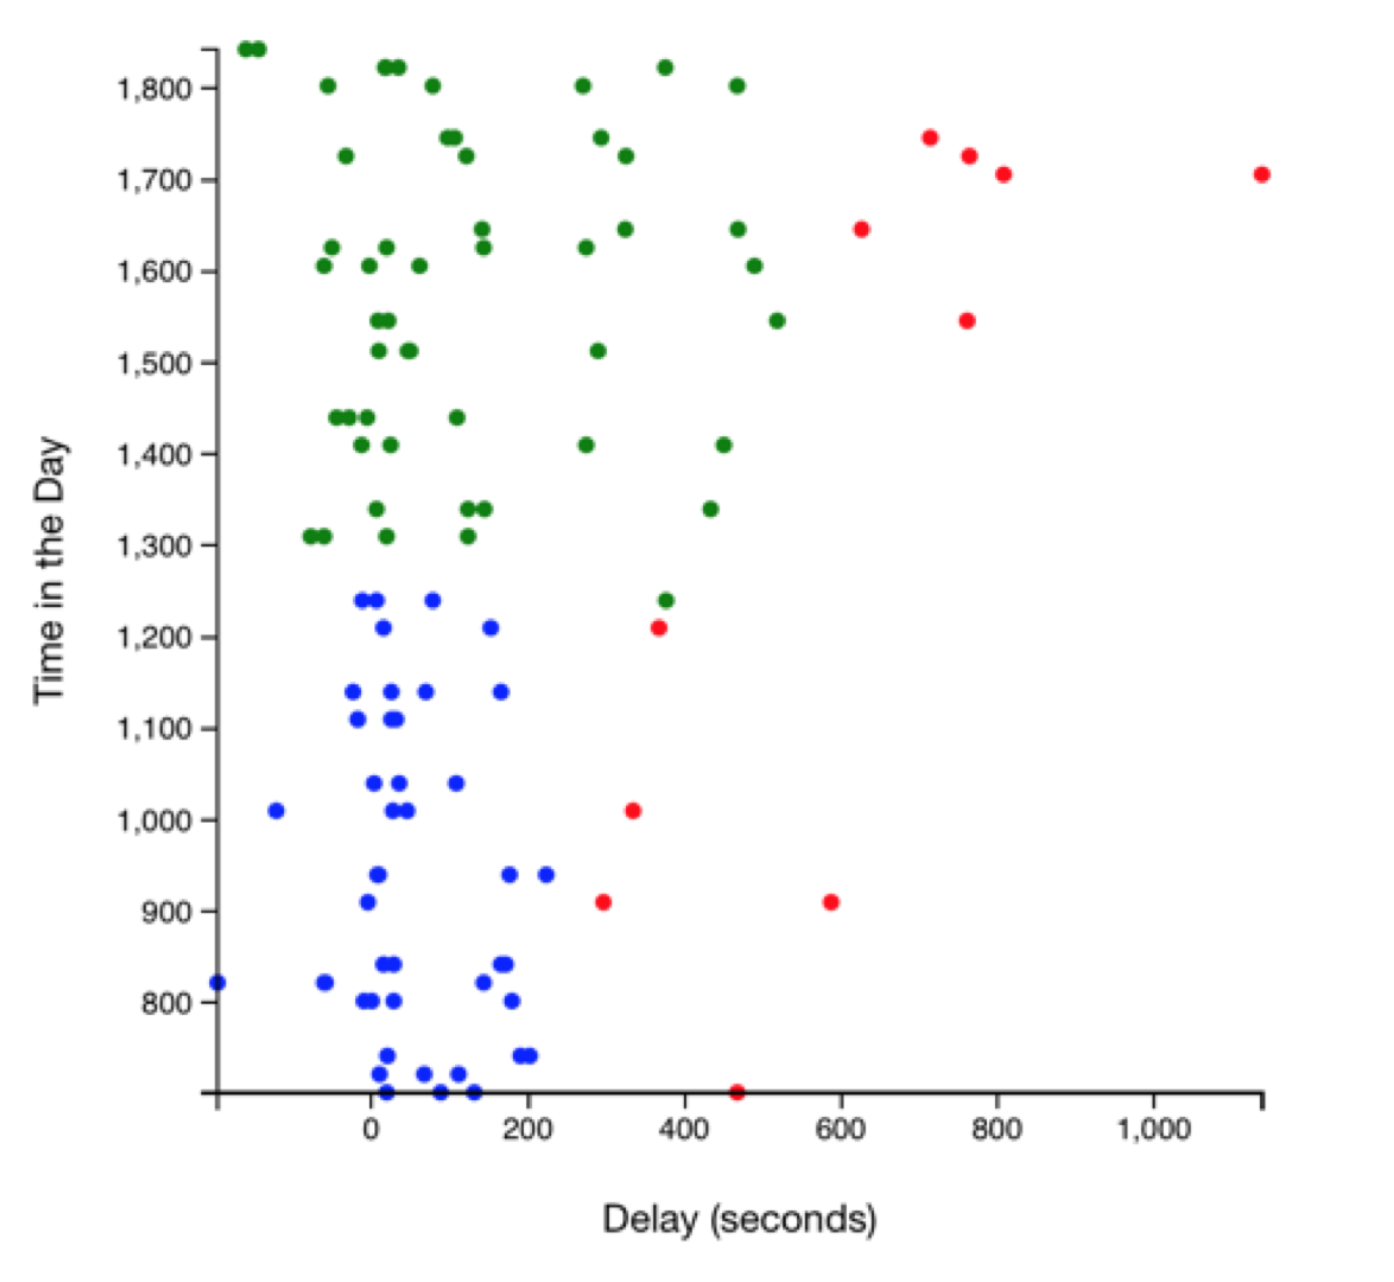
\includegraphics[scale=0.4]{Images/smart-clustering-analysis-1.png}
    \caption{Clustered historical delay data, original image from \cite{smart-public-transport}}
    \label{fig:clustered-historical-data}
\end{center}
\end{figure}

F. Sun et al.'s results support the hypothesis that time of day does affect the delay, and thus arrival time of a bus. Therefore, this parameter is worth investigating further in this project. See Section \ref{time-of-day-week} for further discussion on time of day and week as a parameter affecting bus arrival times. 

We can see that this method of clustering data acts as a good way of deciding which of the parameters that could affect bus arrival times are worth pursuing further. 

\subsection{Regression}

Univariate and multivariate regression models have been used to predict bus travel times. These models are able to work satisfactorily even if traffic conditions are not stable and therefore, would be a good choice to try out as one of the models to explore. However, regression models are generally outperformed by other types of models \cite{dynamic-gps}.\\

Patnaik et al. developed a set of regression models to estimate the arrival times for buses travelling between two points. They used data collected by automatic passenger counters (APC) installed on buses in North-East United States of America \cite{apc-estimation}. For their model, they chose the following variables as independent variables: distance, number of stops, dwell times, number of boarding and alighting passengers and weather descriptors. To decide whether a model was reasonable, Patnaik et al. looked at the values of the $R^2$ and the correlation between the variables and analysed the residuals. The results of these investigations indicated that weather was not a significant factor for estimating bus arrival times (see Section \ref{weather} for a further discussion on this). Other findings from this investigation were that trips taking place on different days of the week (excluding weekends) did not contribute any measurable difference to the travel, whereas time of day appeared to affect travel time significantly. The effect of time of day and time of week is discussed further in Section \ref{time-of-day-week}.

\subsection{Kalman Filters}

Kalman filtering has been a popular choice of model for those researching bus delay predictions because of its capacity of filtering noise and its dynamic nature. \\

Fan and Gurmu studied Kalman Filters as one of three models for predicting bus arrival times \cite{dynamic-gps}. They used the mean absolute percentage error (MAPE) to evaluate the performances of their models (See Section \ref{evaluation} for more details) and discovered that the Kalman Filtering model gave a better prediction in most of the time intervals. It was hypothesised that this was because the model always uses the current measurement to predict the next step. However, the model was found to be vulnerable where there were huge differences in travel times between two consecutive time periods, perhaps because it struggled to filter out noise as smoothly and so was not as capable of handling abrupt changes between consecutive travel times. \\

Sun et al. also used a Kalman Filter model to analyse their data for real-time bus arrival time predictions \cite{smart-public-transport}. To evaluate their results, the root mean square deviation (RMSD) of delay predictions was used (Equation \ref{eq:rmsd}):

\begin{equation}
    RMSD = \sqrt{\frac{\sum (t_{arr}^{act} - t_{arr}^{pred})^2}{n}}
    \label{eq:rmsd}
\end{equation}

where $t_{arr}^{act}$ is the actual arrival time, $t_{arr}^{pred}$ is the predicted arrival time and n is the number of bus trips in the data set. They discovered that as the length of time from which the historical real time data is used (e.g. using the data collected from the past two hours as opposed to historical data from last week), increases from 30 minutes to 90 minutes, the model has a vast improvement on accuracy. However, the performance increase begins to plateau as the length of time increases any further, with the model flat lining when the time window goes beyond 120 minutes. This indicates that only data within the last 120 minutes is significant for real time delay prediction. It was also discovered that the prediction performance of the models worsened as the prediction is applied further in the future. 

\clearpage